\chapter{The Proposed System}
\label{sec:proposedSystem}
\section{Aims of the System}
\label{sec:AimsOfTheSystem}
The previous chapter showed the current trends in sketch recognition. This thesis introduces a new approach for the sketch recognition problem. Particle Swarm Optimization (PSO) is used to correctly segment strokes into curves and lines. Particle Swarm Optimization (PSO) is used to correctly segment strokes into curves and lines. The current implemented systems either segment strokes based on simple curvature\cite{meanshift10,earlySketchbased4} or speed information\cite{earlySketchbased4}. %the performance of most algorithms is based on user style. 

% Stroke segmentation is one of the most complex problems in the sketch recognition system. It is dividing the   
%In stroke segmentation problem is Particle swarm optimization is used as the 

\section{System Overview}
\label{sec:AnOverviewOfTheSystem}
   This research solves sketch segmentation problem using particle swarm algorithm PSO.  Due to sloppiness of users and hardware glitches the captured points must be processed to remove noise and redundancy before the system proceeds to compute the speed and curvature information. After that a set of possible corner or critical points is computed to guide the segmentation procedure.  A set of features is extracted from the segmented strokes to be used by the classifier.  %The stroke is the path of points from the instant the pen is down till it is up.
The block diagram in Figure \ref{fig:Blockdiagram} shows the main system blocks. The next section describes each block in details.
 %Due to sloppiness of users and hardware glitches the system processes the data before further
\begin{figure}[]
	\centering
	
\begin{center}
	\includegraphics[scale=0.75]{images/AllBlockDiagram.eps}
	\caption[The System Block Diagram]{The block diagram of the system}
	\label{fig:Blockdiagram}
\end{center}
\end{figure}
 

%\subsection{System Components}
%\label{sec:SystemComponents}

The \textbf{preprocessing} step is  is responsible for capturing the input data and removing the noise from it. As shown in Figure \ref{fig:Blockdiagram} preprocessing consists of computing the time differences, direction, speed and curvature of every point in the stroke. After computing this information the local minimum and local maximum of each curve is extracted. This process estimates a set of a set of Possible Dominant Points $P_{pd}$ that guide the segmentation process. Later, other geometrical and statistical computations are evaluated from the stroke. %The system then proceeds to estimate to help in the segmentation process.   \\
 
  
The next step is \textbf{Segmentation}, the goal of the segmentation stage is to divide strokes into segments of either curves or lines. As shown in Figure \ref{fig:Blockdiagram} first an attempt is made to fit the stroke points into a curve or an ellipse using a minimum square error fitting algorithm \cite{chernov-2003}. If the stroke proved to be an elliptical arc then the segmentation process ends and the system proceeds to the next step. Otherwise, the stroke is passed to two particle swarm algorithms that divide the stroke to either a polygon or a set of lines and curves. The algorithms takes the stroke points along with the possible dominant points $P_{pd}$ computed during preprocessing then produce a set of dominant points which are connected by either lines or curves. The two algorithms will generate two segmentations, the system will choose the segmentation that has the minimum segmentation error.%
% First an attempts the segmentation process is divided into two steps ellipse fitting and curve segmentation. In the first step, the ellipse fitting process tries to fit the stroke into an ellipse. If the system fails it passes the stroke to the second step; curve segmentation which consists of two PSO segmentation algorithms. The two algorithms will generate two segmentations, the system will choose the segmentation that has the minimum segmentation error.%  generate the segmentations,  the minimum error will be the chosen segmentation. % is the ellipse fitting

 %the stroke first If the ellipse detection fails the stroke is passed to the segmentation algorithms which will pass it to the two PSO algorithms described below the segmentation with the minimum error will be the chosen segmentation.  The segmentation is then added to the set of un-recognized segments in the system. \\% this part is repeated for each stroke. 
 %the clustering algorithm starts to group segments together after the segmentation step. The system let the user draws the symbol by using any number of strokes, a set of unrecognized segments is passed to the clustering algorithm to generate a symbol and compute a feature vector for it.
 
 In \textbf{Feature Extraction} step, a feature vector consists of a set of statistical, geometrical and spatial features is extracted from the segmented strokes. The feature vector is used as input for the next step.   %the system computes composite set of features some are statistical other are spatial features based on the type primitives.% The system extract segment based and statistical based features from the set of segments that the clustering algorithms produce. 
  
   The final step is \textbf{Classification} using a SVM classifier. The classifier attempts to classify the symbol into one the previously trained classes.% c  that will use the features computed to classify the segments into one of the previously trained classes. % Or to determine the symbol of the given segments from the set of preciously trained symbols. 
 
 %with a symbol from the training set.% The system compute composite set of features some are statistical other are spatial features based on the type primitives. Finally, the strokes are classified into the corresponding classes.% the classifier identifies the strokes into a symbol from the set of known symbols.\\

%\chapter{System Details}
%\label{sec:SystemDetails}


\section{Preprocessing}
\label{sec:Preprocessing}
%Some data is extracted from the points in the stroke.
The preprocessing step captures the points from the pointing devices then compute the information needed to determine a set of  \textit{Possible Dominant Points $P_{pd}$} which guides the segmentation step. It is noted as a person draws a shape the pen slows down near corners and picks up speed when drawing straight lines. Therefore, the speed information is widely used to identify the shape corners and edges \cite{earlyprocess}. The curvature information is used to determine the points with high angular changes along the path of points \cite{meanshift10}. Those observations help detecting the dominant points as the points with lower speeds and high curvatures. 

Also the time difference between samples was used in \cite{polygonfeedback31} as it provides more distinct maxima than the speed information. Agar et al. \cite{polygonfeedback31} mentions that the pointing device (for example the mouse) sampling rate is the reason for this phenomena. The points are sampled at regular time intervals while the pointing device is moving. There are no points while the pointing device is stationary. This leads to a nearly constant time difference between samples while the pen is moving and large difference while the pen is stationary. Contrary to speed information, where the users draw with variant speeds the speed information has a lot of noise in the data. Figure \ref{fig:speed2Distance} shows the time difference and the speed graphs for the stroke drawn in Figure \ref{fig:orignalStroke}.  Similarly, direction information is used as it provides better distinctive maxima for the corners than the curvature information \cite{meanshift10}. Figure \ref{fig:curvatures} shows the direction and curvature graphs for the stroke drawn in Figure \ref{fig:orignalStroke}

 %The system compute speed, curvature, time difference and direction data then generate a set of possible corners that will be used in the segmentation as an initial solution. 
\subsection{Preliminary Calculation}
\label{sec:CurvatureCalculation}
  
 
 In this research, time difference, direction, speed and curvature of each point along the stroke was computed. The experiments in section \ref{} proved that computing all information's provide better segmentations results than only using one of the graphs. The time difference is calculated as $\Delta t = t_{i+1} - t_i$ where $t_i$ is the time of the point $i$ and $t_{i+1}$ is the time of the point $i+1$. The speed is calcuated using equation $v=\Delta s/\Delta t$ where $t$ is the time difference between two points and $s$ is the length between them. 
 
\begin{equation}
\label{eq:direction}
	\vartheta  = \cos ^{ - 1} \left( {\frac{{\overrightarrow {p_1 p_2 }  \cdot \overrightarrow {p_2 p_3 } }}{{\left\| {\overrightarrow {p_1 p_2 } } \right\| \times \left\| {\overrightarrow {p_2 p_3 } } \right\|}}} \right)
\end{equation}



  The direction is calculated as the angle between two vectors as in equation \ref{eq:direction} where $\overrightarrow {p_i p_j }$ is the vector from point $pi$ to point $pj$ and $\|{\overrightarrow {p_i p_j }}\|$ is the normal of the  vector $\overrightarrow{p_i p_j }$. The curvature is estimated using more than one method the result of each curvatures estimation is reported in section \ref{sec:Curvatureestimationresults}. The best curvature estimation is used, the estimation define curvature as the change in direction with respect to length i.e. $c= \Delta d/\Delta s$.
 
 %system compute speed, distance data for all points in the stroke. Curvature is computed using estimation used in [] where direction computed is angle between two lines. Curvature is 
 %$\Delta d/  \Delta S $ where d is the difference direction of point and s is difference in distance between points. 
 All these calculations are performed in real time while the user draws the strokes. The complexity of computation is $O(n)$ where $n$ is number of points. Figures \ref{fig:speed2Distance} \&  \ref{fig:curvatures} show the computed information's for the stroke drawn in Figure \ref{fig:orignalStroke}.% After computing the graphs the system  compute the average, minimum and maximum values of all curves.  \\% the lower speed points correspond to vertex and dominant point's location. The higher the direction and curvature data correspond to location with higher change in curvature witch promote the location for vertices'. \\
%Description of input data. 
%how to calculate speed, curvature, area, bounding box.
%how to remove noise. 
%Finally how to compute primarily dominant points. 

\begin{figure}[]
	\centering
		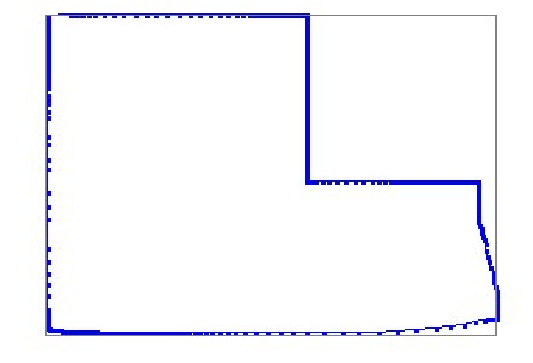
\includegraphics[scale=0.8]{images/orignalStroke.eps}
	\caption{Input Stroke} Example of an input stroke to the system. 
	\label{fig:orignalStroke}
\end{figure}


\begin{figure}
	\centering
			\subfigure[ Speed Graph]{	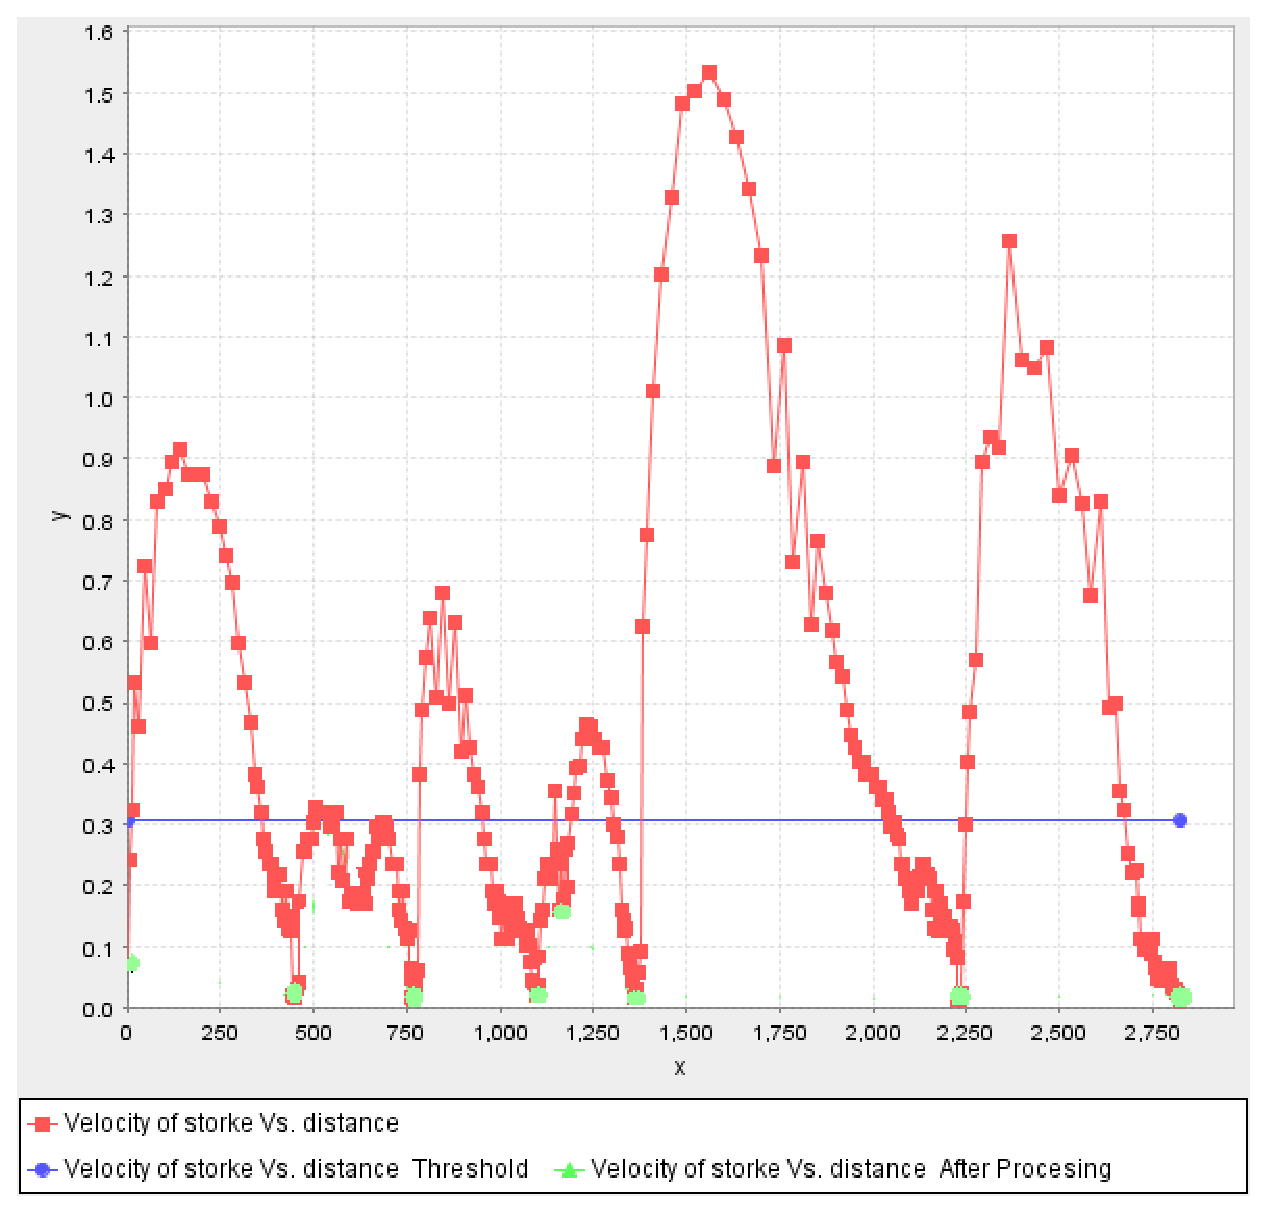
\includegraphics[scale=0.5]{images/speed2.eps}}
			\hfill
			\subfigure[ Time Difference Graph] {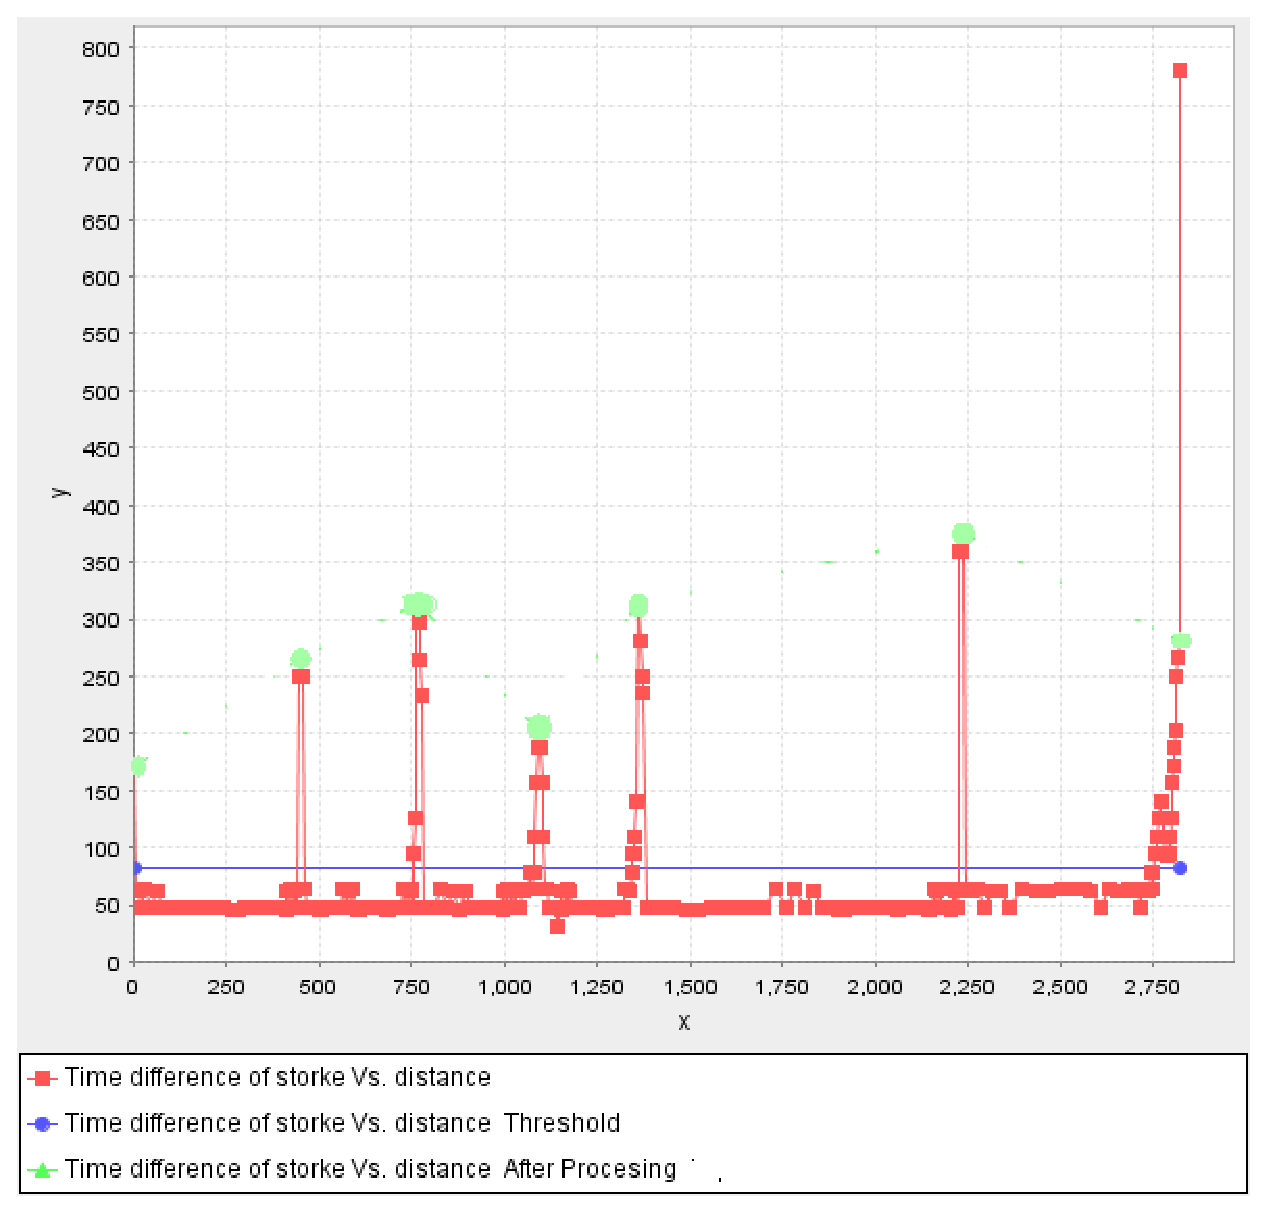
\includegraphics[scale=0.5]{images/time2.eps}}
	\caption{Speed and Time Difference Graphs}
	\label{fig:speed2Distance}
\end{figure}



\begin{figure}[]
%\begin{minipage}[b]{0.8\linewidth}
	\centering

	%	\subfigure[ The Speed of data] {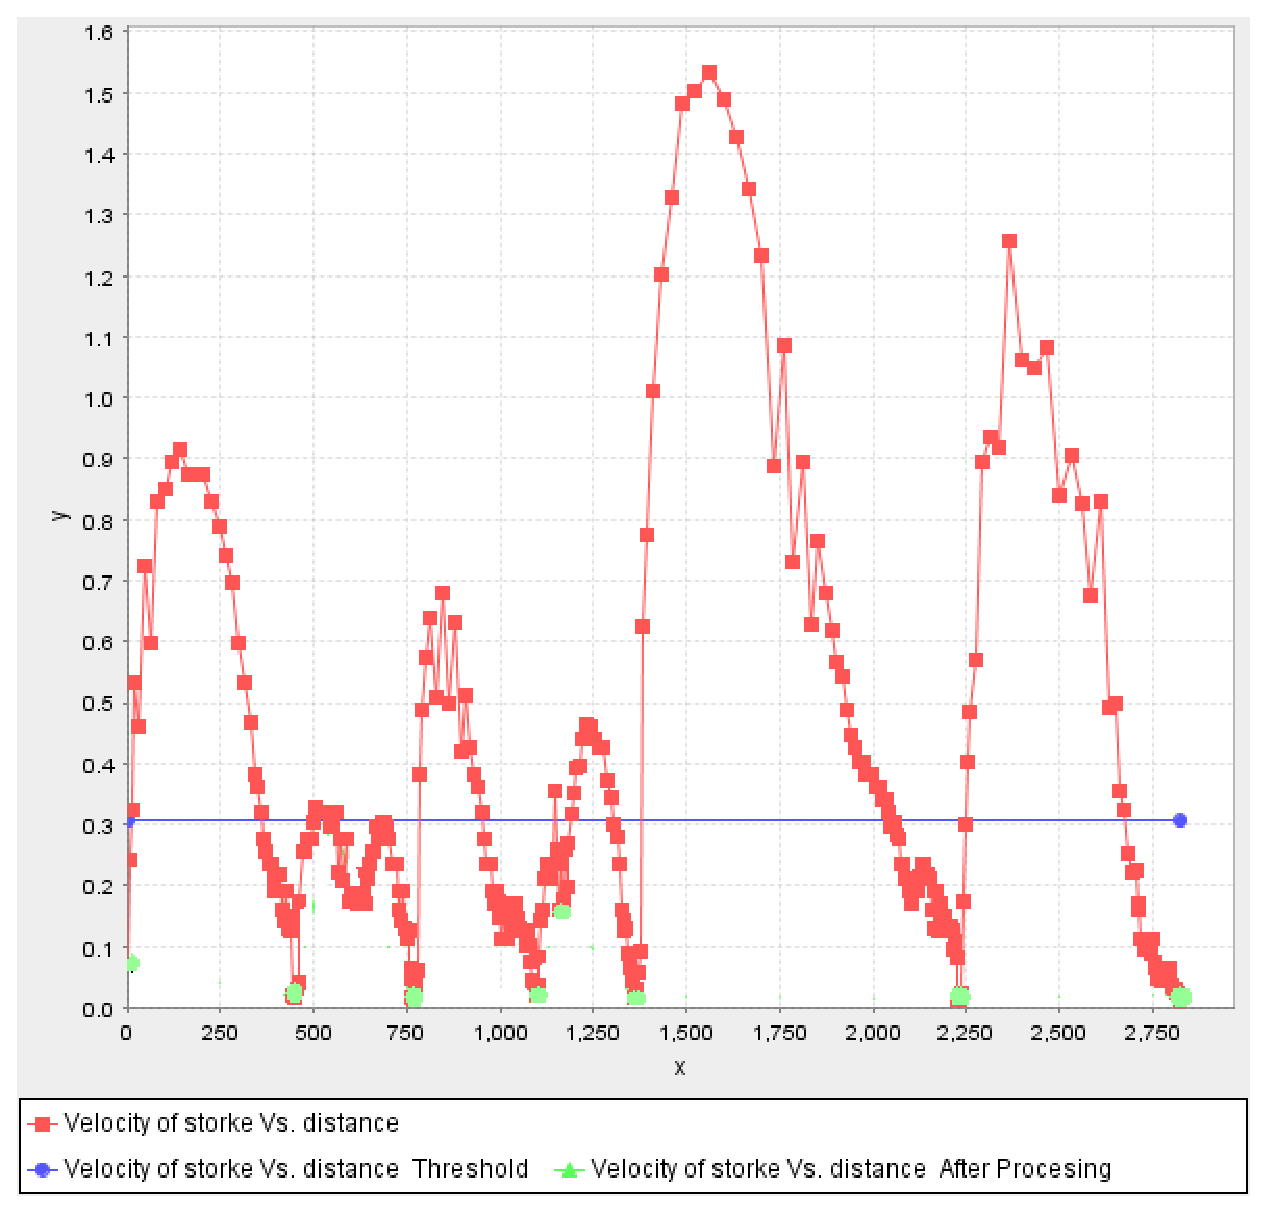
\includegraphics[scale=0.35]{images/speed2.eps}}
		
		\subfigure[ Direction Graph ] {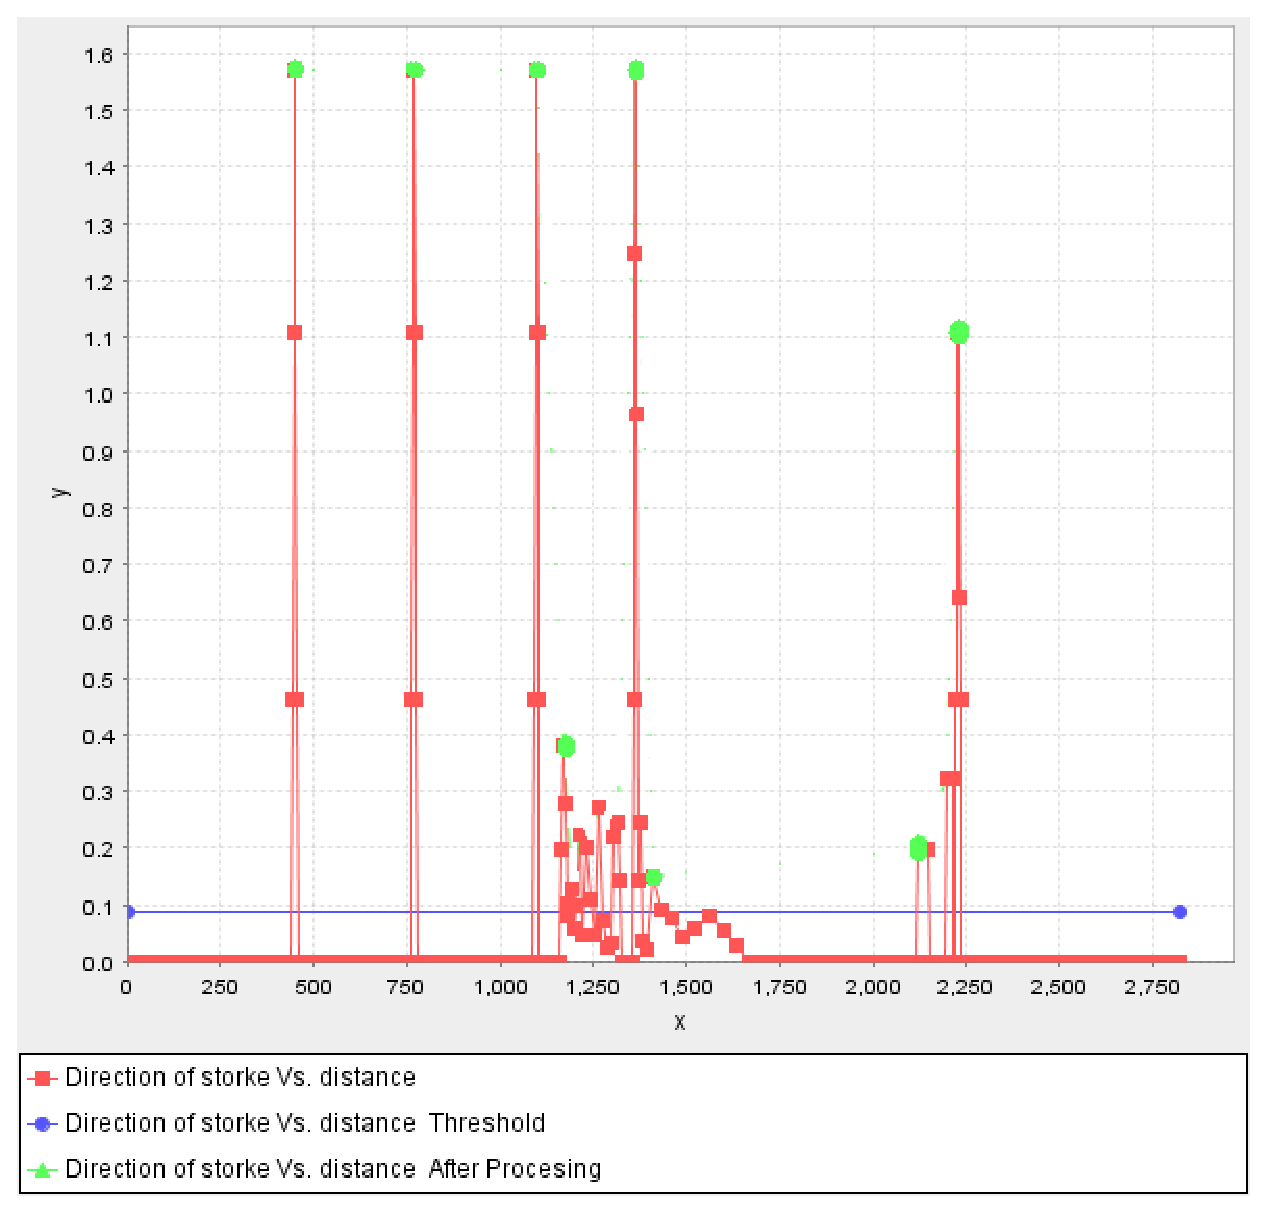
\includegraphics[scale=0.35]{images/direction2.eps}}
					%\end{minipage}
					%\begin{minipage}[b]{0.8\linewidth}
			\subfigure[Curvature Graph] {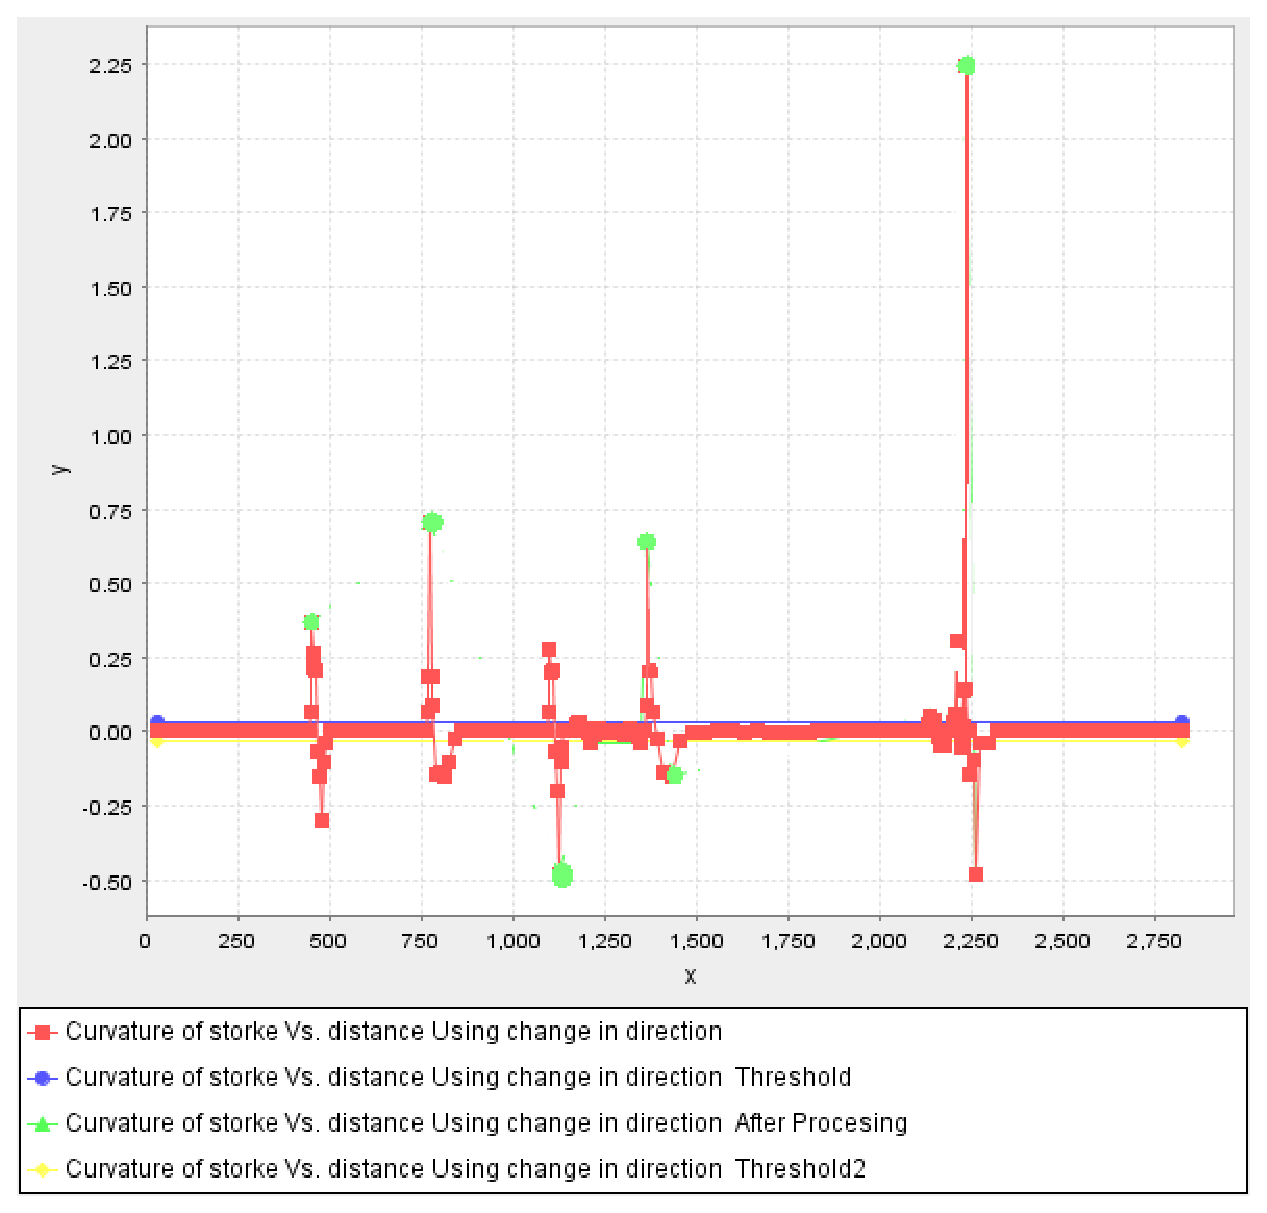
\includegraphics[scale=0.35]{images/curvature2.eps}}
		
			%\end{minipage}
	
	\caption{Curvature and Direction Graphs}%{The data of the stroke}
	
	\label{fig:curvatures}
\end{figure}


\subsection{Critical Point Detection}
\label{sec:CriticalPointDetection}
After computing speed, time difference and curvature information the system proceeds to detect the points with low velocity and high curvatures. Using simple differentiation to detect local extreme points resulted in false points due to the non smooth curves. Hence, the system adopted a process presented by \cite{earlyprocess}, where the mean of the curve is calculated. Then a threshold \textit{th} is used to separate the curve into regions; each region $Region_i$ is defined as a range of points, where the curve values are either above or below the threshold \textit{th}. Those regions are further processed to find the maximum point $Max(Region_i)$ of each region $Region_i$. The stroke points $p_i(x,y)$ that correspond to those maximum values are labeled as \textit{possible dominant points} $P_{pd}$. Figure \ref{fig:MaxRegioi} shows an example of $Region_i$ of the speed curve and the dominate points $P_{pd}$ which correspond to the minimum of point in this region $Min(Region_i)$.  % (as shown are redundant)
\begin{figure}
	\centering
		\includegraphics[scale=0.5]{images/speedreg.eps}
	\caption{Possible Dominant Points Calculations}
	\label{fig:MaxRegioi}
\end{figure}

   %After the threshold is applied the curve is divided into regions. Each region is defined by a part in the data curve between tow intersection point of the threshold line and the curve.  % to find the extreme points. Hence, the mean of the direction curve is calculated and used as threshold.   \\
   %If we tried to differentiate the curve the result will be false threshold values we divide the data into regions of data higher or lower that the threshold. This will let us only look for high data only. The maximum of each region is then computed and reported as a possible vertex point. 
  
The system repeats this process to curvature, direction, time difference and speed curves. For each curve the points labeled as possible dominant points $P_{pd}$ are saved into a single array. The points that are repeatedly labeled are given a higher score than the other points. This score is then used to sort the  $P_{pd}$ points array. The array that contains possible points $P_{pd}$ is used as input for the next segmentation step. Figure \ref{fig:LabelsPPD} shows the particles labeled as Possible dominate points $P_{pd}$ by the preprocessing, it is noticed the redundancy of some $P_{pd}$ points. 


\begin{figure}
	\centering
		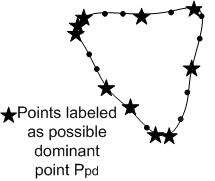
\includegraphics{images/ppd.eps}
	\caption{Posible domninate points}% a) Possible dominate point b) Particle encoding  
	\label{fig:LabelsPPD}
\end{figure}

\section{Segmentation}
\label{sec:Segmentation}
The segmentation tries to divide the stroke into a set of primitives. As shown in Figure \ref{fig:Blockdiagram} first an attempt is made to fit the stroke points into a curve or an ellipse using a minimum square error fitting algorithm \cite{chernov-2003}. If the stroke proved to be an ellipse arc then the segmentation process ends and the system proceeds to the next step. Otherwise, the stroke is passed to two particle swarm algorithms that divide the stroke to either lines or lines and curves. The algorithms take the stroke points along with the possible dominant points $P_{pd}$ computed during preprocessing then produce a set of dominant points which are connected by either lines or curves. The next section describes the ellipse detection algorithm and the two particle swarm algorithms used to divide the stroke.
%If the stroke proved to be an ellipse then the segmentation process ends and the system proceeds to the next step. Otherwise, the stroke is passed into two particle swarm algorithms that will divide the stroke to either lines or lines and curves (see the block diagram in fig. \ref{fig:Blockdiagram} ). 
%The algorithms takes the stroke points along with the possible dominant points computed then produce a set of dominant points which are connected with either lines or curves (see fig. \ref{fig:Blockdiagram}).  The next sections will describe the ellipse detection algorithm and both the two particle swarm algorithms used to divide the stroke.
%After computing the primary data the system now tries \\
%Paragraphs describe the segmentation algorithm.  


\subsection{Ellipse Fitting }
\label{sec:EllipseDetection}
%Describe the ellipse detection algorithms 
This process tries to fit the stroke points into an ellipse arc; it starts with computing the center of the stroke bounding box. The bounding box center point is used as the first estimation of the center of the ellipse. The axes of the ellipse are estimated as the $w/2$ and $h/2$ of the stroke bounding box where $w$ is width and $h$ is height of the bonding box. The least square fitting algorithm \cite{chernov-2003} is used to minimize the fitting error of the ellipse Equation (\ref{eq:circleFit})  

\begin{equation}
E = \sum\limits_{i = 0}^N {\frac{{(x_i - x_0 )}}{{a^2 }}^2  + \frac{{(y_i - y_0 )}}{{b^2 }}^2  - 1} 
\label{eq:circleFit}
\end{equation}

 where $N$ is number of points in the stroke, $a,b$ are the length of ellipse axes, $x_0$ \& $y_0$ are the coordinates of the center point, $x_i$ \& $y_i$ are the coordinates of point $i$ in the stroke. A list of new values for $x_0$ , $y_0$ ,$a$ and $b$ are generated randomly from the older values with small increments after each loop. After few loops, the final fit error and the ellipse confidence value are computed. The confidence value $Conf$ computed by Equation (\ref{eq:circleError})
 \begin{equation}
Conf = E_{ellipse}+E_{area}
\label{eq:circleError}
\end{equation}
 \begin{equation}
E_{area}  = \sqrt {\left( Area(stroke) - Area(ellipse)\right)^2 }
\label{eq:ErrorArea}
\end{equation}

   where $E_{ellipse}$ is the error computed by Equation(\ref{eq:circleFit}) and $E_{area}$ is computed as the difference between the actual area of the stroke and the area of the estimated ellipse Equation(\ref{eq:ErrorArea}). If confidence value $Conf$ is less than threshold $th_{Ellipse}$\footnote{ Using trial and error the best threshold used is $th_{Ellipse}=0.7$ } the stroke is segmented as an ellipse otherwise the system proceeds to the two DPSO segmentation algorithms.  % The confidence value is used to label the stroke as ellipse or un segmented stroke. If the stroke as un-segmented the next process will be to pass the stroke into curve segmentation algorithm.    
   
 %  The next section describes the \textit{Discrete Particle Swarm Algorithm (DPSO)} then it proceeds to detail the two DPSO segmentation algorithms. 
   
   %to check if the stroke can be labeled as ellipse or not.\\ %is computed to check if stroke is an ellipse. \\
%We found that if the confidante is above threshold then the probability of ellipse is highest otherwise the stroke is passed to the next section to get the divisions of stroke and test its error.  


%\subsection{Discrete Particle Swarm Algorithm}
%\label{sec:ParticleSwarmAlgorithm}
%%\section{Particle Swarm Algorithm}
%%\label{PSO}
%%What is particle swarm algorithm and how it was used in related researches. 
%The main idea of \textit{Particle Swarm Algorithm (PSO)} is to represent each agent with a particle from the solution space \cite{PSOFirst}. Each agent moves the particle with a direction and velocity $v_{ij}$ based on equations \ref{eq:Swarm} \& \ref{eq:Swarm1}.
%\begin{equation}
%%\[
%p_{ij}=p_{ij}+v_{ij},
%%\
%\label{eq:Swarm1}
%\end{equation}
%where $p_{ij}$ represent the $jth$ particle in the $ith$ agent and $v_{ij}$ is the velocity of the $jth$ particle in the $ith$ agent.
% %Equation [\ref{eq:Swarm}] shows how velocity and direction of each particle are computed
% \begin{equation}
%v_{ij}  = v_{ij}  + c_1 r_1 (lbest_{ij}  - p_{ij} ) + c_2 r_2 (gbest_{ij}  - p_{ij} )
%\label{eq:Swarm}
%\end{equation}
% where $lbest_{ij}$ is the local best particle, $gbest_{ij}$ is the global best particle, $r_1$ \& $r_2$ are random variables and $c_1$ \& $c_2$ are the swarm system variables.
% After each iteration the global best $g_{best}$ particle and the agent local best $l_{best}$ particle are evaluated based on the maximum fitness functions of all particles in the solution space. The solution is found after achieving a specific number of iteration or after an error threshold is achieved.
%Equation \ref{eq:descrite}  
%\begin{equation}
%   P(i)\Leftarrow 
%\{
%\begin{array}{c} 
%1 \quad \quad if\quad r_{3}>p_{i}  \\
%
%0 \quad \quad if\quad r_{3}<p_{i} 
%\label{eq:descrite}
%\end{array}\}
%\end{equation}
% where $p_{ij}$ is the numerical values of the particle and $r_{3}$ is a random variable, is used to change the general swarm algorithm into binary particle (\textit{Discrete Particle Swarm Algorithm DPSO}) which handles particle values of either $0$ or $1$ \cite{PSODisceret}.  
\subsection{Swarm Segmentation}
\label{sec:SwarmSegmentation}
Two DPSO algorithms generate two different segmentations for each stroke. Each DPSO algorithms tries to find the best particle in the solution space. Both algorithms has the same problem formulation but different fitness functions. After generating two segmentations the system chooses the best segmentation from the outputs of the DPSO. The details of the problem formulation and fitness functions are given in the following sections.
%In this process the system generate two stroke segmentation using two PSO segmentation algorithm. The system generates segmentation from both algorithms and then chooses the segmentation with the minimum error value. The problem definition is the same in both algorithms but they differ in the fitness function and the error functions. %formation is nearly the same in both. 
\subsubsection{Problem Formulation}
\label{sec:ProblemFormulation}
The input stroke with $N$ points can be represented by set $S = \left\{ {x_1 ,x_2  \ldots x_N } \right\}$ where $x_i$ is the location of the point $i$ . The swarm algorithms consist of $M$ agents which are represented by the set 
$A  = \left\{ {P_i \left| {i = 1,2 \cdots M} \right.} \right\}$ where $P_i$ is a single solution particle from the solution space. Each particle decodes the problem with binary array with the same length $N$ as the input stroke (Figure \ref{fig:CodingSwarm}).   
\begin{figure}
	\centering
		\includegraphics{images/CodingSwarm.eps}
	\caption{An Example Stroke and the Coding}
	\label{fig:CodingSwarm}
\end{figure}
% The particles of the swarm represent a single solution of the solution space. For this problem the, each particle %will give a different segmentation for the input stroke. Firstly, we will define the stroke with N points by the set %S where.  We define the arc %An array with the same length as the number of points of the strokes.
The system represents each particle $P_i$ by $P_i = \left\{ {p_{ij} \left| {j = 1,2 \cdots N} \right.} \right\}$ where $p_{ij}$ is either 0 or 1 where $p_{ij}=1$ means that point $j$ is a dominant point(see Figure \ref{fig:CodingSwarm}.  Thus , the particle represents points that are chosen to be used as dominant points for this segmentation. 
The goal of the DPSO algorithm is to find the solution $P_i$ that generates the minimum set of dominate points that defines the stroke with minimum segmentation error. In other words, the system tries to find the fewer number of points (1's) location in the particle array which gives minimum segmentation error.  


The fitness function and error calculations are different in each algorithm. The first fitness and error function are described below. 


\subsubsection{Polygon Division Algorithm \textsl{AlgS1}}
\label{sec:PolygonDivisionAlgorithm}
The first algorithm, the algorithm tries to segment the stroke as a polygon. The final solution is a set of line segments that best define the input stroke. Given the inputs stroke let's define the set of points in the stroke as  $S = \left\{ {x_1 ,x_2  \ldots x_N } \right\}$ which is the set of consecutive points from start of stroke till the end. The arc $\widehat{x_ix_j}$ is defined as the consecutive set of points from point $x_i,x_{i+1} \cdots,x_j$. The line
$\overline{x_i x_j} $ is the straight line connecting point $x_i$ to point $x_j$. The approximation error is computed by the equation \ref{eq:ErrorSwarm1} 
\begin{equation}
E=\sum\nolimits_{i = 0}^M e ( \widehat{x_ix_{i+1}},\overline{x_i x_{i+1}})
\label{eq:ErrorSwarm1}
\end{equation}
 where $M$ is the number of dominant points in this solution.  The error $ e ( \widehat{x_ix_j},\overline{x_i x_j})$ is computed as the sum of squared perpendicular distance from every point along the arc $\widehat{x_ix_j}$ to the line $\overline{x_i x_j}$ \cite{PolygonApproximationPSO}. Figure \ref{fig:DPSOERROR} shows a graphical representation of the error. The fitness is computed using equation \ref{eq:fitnessSwarm1} 
\begin{equation}
\max fitness(p_i ) = \left\{ {\begin{array}{*{20}c}
   { - E/\varepsilon N} & {ifE > \varepsilon ,}  \\
   {D/\sum\limits_{j = 1}^N {p_{ij} } } & {otherwise}  \\
\end{array}} \right.
\label{eq:fitnessSwarm1}
\end{equation}%\]
where $N$ is the number of points in the stroke, $D$ is the number of point in the solution that was previously labeled as $P_{pd}$  and $E$ is the computed error and $\varepsilon$ is the error threshold.  If the solution produced an error that exceed the error threshold $\varepsilon$ the fitness function assign a -ve value for the solution to express it's in feasibility, otherwise the inverse of the number of vertex produced is used to access the solution fitness in terms of minimum number of vertices'.  This fitness function optimize two goals the first is to move the solution into the feasible solution space with acceptable error bounds and second is to fly the particle to a new position which may result in a polygon with a fewer number of vertices'\cite{PolygonApproximationPSO}. 
\begin{figure}
	\centering
  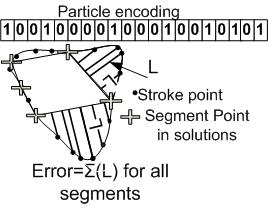
\includegraphics[scale=0.8]{images/pso1.eps}			
	\caption{ALS1 Error}% a) Possible dominate point b) Particle encoding  
	\label{fig:DPSOERROR}
\end{figure}
 %The error is chosen to in favor of larger than the threshold is given a -ve value to lower the value of solution otherwise the system will favor the lower number of vertices'.\\ %we will want to lower the number of vertices'. \\
%if we say that s
%Alg1:
%Alg2: 
\subsubsection{Curve Divisions Algorithm \textsl{AlgS2}}
\label{sec:PolygonDivisionAlgorithm}

The second algorithm has the same problem formulation but different fitness and error functions. It was previously introduced in  \cite{CruveDivisionSwarm} where genetic programming was used as the optimizing algorithm. The particle is represented using the arrays $P_i = \left\{ {p_{ij} \left| {j = 1,2 \cdots N} \right.} \right\}$ where $p_{ij}$ is either 0 or 1. Lets denote the segments $\widehat{x_ix_j}$ as the consecutive set of points from point $x_i,x_{i+1} \cdots,x_j$. The algorithms attempts to fit each segment $\widehat{x_ix_j}$ to both line and circle. The type of the segment is determined according to the minimum error of each fit. The final error of the solutions is the summation of error of all segments.  %The goal of the algorithm is to fit the segments between the solution vertices' into straight lines or a circular arc. 
\paragraph{Fitting segments into straight line.}
\label{sec:FittingSegmentIntoStraightLine}
According to \cite{CruveDivisionSwarm} each segment $\widehat{x_ix_j}$ given a set of points $x_i,x_{i+1} \cdots,x_j$ can be fitted into the line: $y=kx+c$ where $k$ and $c$ are the slope and the intercept of the line respectively. Equation \ref{eq:Linek} and \ref{eq:LineC} 
\begin{equation}
\label{eq:Linek}
k = \frac{{N\sum\limits_{i = 1}^N {x_i y_i }  - \sum\limits_{i = 1}^N {x_i } \sum\limits_{i = 1}^N {y_i } }}{{N\sum\limits_{i = 1}^N {x_i^2 }  - \left( {\sum\limits_{i = 1}^N {x_i } } \right)^2 }}
\end{equation}
\begin{equation}
\label{eq:LineC}
c = \frac{{\sum\limits_{i = 1}^N {x_i^2 } \sum\limits_{i = 1}^N {y_i }  - \sum\limits_{i = 1}^N {x_i } \sum\limits_{i = 1}^N {x_i y_i } }}{{N\sum\limits_{i = 1}^N {x_i^2 }  - \left( {\sum\limits_{i = 1}^N {x_i } } \right)^2 }}
\end{equation}
, where $N$ is the number of points in the segment and $(x_i, y_i)$ are the coordinate of the point $i$, are used to fit the segment $\widehat{x_ix_j}$ into the straight line.
\begin{equation}
\label{eq:ds}
 d_s  = \frac{{\sum\limits_{i = 1}^N {\left| {(kx_i  + c) - y_i } \right|} }}{{N\sqrt {k^2  + 1} }}
\end{equation}
The distance ($d_s$) (Equation \ref{eq:ds}) is the average distance from segment points $(x_i, y_i)$ to the estimated line. This distance $d_s$ is used as the error of the line approximation.
\paragraph{Fitting segments into circular arc.}
\label{sec:FittingSegmentcirculararc}
Each segment is also fitted into a circular arc $(x - a)^2  + (y - b)^2  = R^2, $ where ($a,b$) are the coordinate of the center of the circle and $R$ is the radius of the circle. They is estimated using the following set of equations: 
 
\begin{equation}
a = \frac{{b_{1}a_{22} - b_{2}a_{12}}}{\Delta},
\end{equation}
\begin{equation}
	b = \frac{{b_{2}a_{11} - b_{1}a_{21}}}{\Delta},
\end{equation}
\begin{equation}
R = \sqrt {\frac{1}{N}(\sum\limits_{i = 1}^N {x_i^2 }  - 2\sum\limits_{i = 1}^N {x_i a}  + Na^2  + \sum\limits_{i = 1}^N {y_i^2  - 2} \sum\limits_{i = 1}^N {y_i b + Nb^2 } )} ,
\end{equation}

Where 
\begin{equation}
a_{11}  = 2\left[ {\left( {\sum\limits_{i = 1}^N {x_i } } \right) - N\sum\limits_{i = 1}^N {x_i^2 } } \right]
\end{equation}
\begin{equation}
a_{12}  = a_{21}  = 2\left( {\sum\limits_{i = 1}^N {x_i \sum\limits_{i = 1}^N {y_i } }  - N\sum\limits_{i = 1}^N {x_i y_i^2 } } \right),
\end{equation}
\begin{equation}
 a_{22}  = 2\left[ {\left( {\sum\limits_{i = 0}^N {y_i } } \right)^2  - N\sum\limits_{i = 0}^N {y_i^2 } } \right]
\end{equation}
\begin{equation}
b_1  = \sum\limits_{i = 0}^N {x_i^2 } \sum\limits_{i = 0}^N {x_i }  - N\sum\limits_{i = 0}^N {x_i^3 }  + \sum\limits_{i = 0}^N {x_i } \sum\limits_{i = 0}^N {y_i^2 }  - N\sum\limits_{i = 0}^N {x_i y_i^2 } , 
\end{equation}
\begin{equation}
b_2  = \sum\limits_{i = 0}^N {x_i^2 } \sum\limits_{i = 0}^N {y_i }  - N\sum\limits_{i = 0}^N {y_i^3 }  + \sum\limits_{i = 0}^N {y_i } \sum\limits_{i = 0}^N {y_i^2 }  - N\sum\limits_{i = 0}^N {x_i^2 y_i } ,
\end{equation}

\begin{equation}
\Delta  = a_{11}b_{22}-a_{12}a_{21}.
\end{equation}
 The error of the circle estimation is measured using the distance $d_c$ which is calculated using equation \ref{eq:circleE}:
 \begin{equation}
 \label{eq:circleE}
d_c  = \frac{{\sum\limits_{i = 0}^N {\left| {\sqrt {(x_i  - a)^2  + (y_i  - b)^2 }  - R} \right|} }}{N}
\end{equation}
Thus, Equation \ref{eq:circleE} $d_c$ defines the average distance $d_c$ from the segment points $x_i,y_i$ to the estimated circle ($a,b$) and $R$.

\paragraph{Determinig The Segment Type.} 
\label{sec:DeterminigSegmentType}
If the average distance $d_s$ equals zero this means that the segment$\widehat{x_ix_j}$ points is exactly the straight line approximated. If the distance ($d_c$) equals zero means that the segments point lies exactly on the circular arc estimated. But the user rarely draws an exact line or circle, so the distances are used as the fitting error. The minimum distance determines the type of the current segment, in other words if ($d_s$) is smaller than ($d_c$) then the segment is labeled as a line segment otherwise it is labeled as a circular arc. 


After each segment type is determined the the particle segmentation error is computed by Equation \ref{eq:errorSwarm2} 
\begin{equation}
E=\sum\nolimits_{i = 0}^M e(D_i) 
\label{eq:errorSwarm2}
\end{equation}
where $M$ is the number of segments in the solution, $D_i$ is the  approximation error of each segment as $min(d_c,d_s)$ as computed in Equation\ref{eq:circleE}  and Equation \ref{eq:ds} \cite{CruveDivisionSwarm}. The fitness is computed by the equation \ref{eq:fitnessSwarm2} 
\begin{equation}
\max fitness(P_i ) = \frac{1}{{E \times M^k }}
\label{eq:fitnessSwarm2}
\end{equation} where $E$ is the error and $M$ is number of segments and $k$ is a parameter tweaked to get minimum number of segments. $k$ is selected to be 0.5\cite{CruveDivisionSwarm}. 

\subsubsection{Solution Refine procedures } 
%\cite{PolygonApproximationPSO} used a merge and divide algorithm after each loop of the swarm system to refine the solution but we used another enhancement method.
 After each loop in the swarm algorithm, each particle loops on the set of selected dominant points to enhance the solution. Each dominant point is checked to find if it was labeled before as a possible dominant (computed as in section \ref{sec:Preprocessing}), if not the point is moved to the nearest labeled point.
   After each loop of the swarm algorithm (\textsl{AlgS1} and \textsl{AlgS2}), each particle is refined using the following procedure. For each particle $P_i$ each dominant point $P_{ij}$ is checked to find if it was labeled before as a \textit{possible dominant point} $P_{pd}$ (computed as in section \ref{sec:Preprocessing}). If it was not labeled the point $P_{ij}$ is moved to the nearest labeled point. This ensures that all of the points generated by the DPSO are possible dominate points $P_{pd}$. After that the particles are tested to make sure that the distance between every two successive dominate point is larger than the constant $min_D$. If two points are nearer than $min_D$\footnote{Constant selected to be 10 pixels} then one of the points is removed. 
\subsection{Choosing the best fit}
The two PSO algorithms produce two segmentation solutions. After that the system evaluates each solution to finally select the best segmentation. This evaluation is based on the area of both the segmentation and the input stroke. Equation \ref{eq:bestFit1} and \ref{eq:bestFit2} are used to evaluate each segmentation.
 
\begin{equation}
\label{eq:bestFit1}
E_{area}=A_{st}-A_{sg}
 \end{equation}
 \begin{equation}
\label{eq:bestFit2}
E_{tot}=E_{area}+E_{alg}
 \end{equation}
 where $A_{st}$ is the area of the input stroke, $A_{sg}$ is area of computed segmenation, $E_{alg}$ is the approximation error of the segmentation. The segmentation which crosspond to the minimum $E_{tot}$ is the best segmentation.  
\section{Hybird Segmentation Algorithm}
\label{sec:BenchMarckAlgorithm}

In this research, we developed another algorithm as reference to the results obtained by the DPSO algorithms. The algorithm was first implemented by  Sezgin et al. in \cite{earlyprocess}. The algorithm is divided into the following steps: 
\begin{enumerate}
	\item Compute the curvature and the speed for each point in the stroke. 
	\item   A percentage of maximum value of the speed and curvature is used as threshold.
		\item Mark the values higher than the threshold in a new arrays $L_c$ as the list of corner points generated from the curvature curve. The list $L_s$ contains the points generated from the speed curve.
	\item Compute a confidence on each list based on the type of curve. Then sort the lists $L_s$and $L_c$ by the confidence value. 
	\item Find the intersection points in both list and generate the a Sample solution $h_{curr}$. 
	\item Use $h_{curr}$ as initial solution. Loop doing the following:
	
		\begin{enumerate}
			\item Generate a new solution $h_{s}$ using $h_{curr}$ and  the first point in the $L_s$ list .
			\item Generate a new solution $h_{c}$ using $h_{curr}$ and  the first point in the $L_c$ list.
			\item Test the solutions $h_{s},h_c$ to find the minimum solution.
			\item  If $h_s$ is the minimum then add the solution a list of hybrid solutions $Solutions_{set}$ and remove the first point from the list $L_s$ then set $h_s$ as $h_{curr}$. 
			\item If $h_c$ then add the solution a list of hybrid solutions $Solutions_{set}$ and remove the first point from the list $L_c$ then set $h_c$ as $h_{curr}$. 
		\end{enumerate}
		\item Choose the final solution from the list of solutions $Solutions_{set}$ as a tradeoff between  minimum error and number of corners.  
		\item Check each segment in the solution if the solution is can be estimated as a line segment if not it is fitted using a higher level Bezire curve. 
\end{enumerate}
More details about the algorithm are in \cite{earlyprocess}.


%\section{Stroke Clustring Algoirthm }
%\label{sec:ClustringAlgoirthm}
%
%When the user finishes drawing a stroke the segmentation algorithm generate a list of segments that represent this stroke. The system then groups the segments generated from the segmentation algorithm. %These segments are grouped into a symbol and tested if they can be classified into one of the known symbols. If no identification is achieved the segments are added into a list of unclassified segments. When a user draws another stroke the segmented stroke is added to the list and the process is repeated until all the segments are classified to a known symbol.\\
%
%After the user draw all strokes of the symbol he has to wait 10 seconds or press finish button beside the drawing area. The set of unrecognized strokes is grouped together along with their segmentation as input to the feature extraction process. 

\section{ Feature Extraction}%%Feature Set
\label{sec:FeatureExtraction}

The system uses a composite set of features include Rubine feature set \cite{gestureexample12}, Zernike moments \cite{HeloiseBeautification}, ink density \cite{GeometryAndDomain102} and some structural information like number of perpendiculars lines , number of parallel lines and types of primitives in each symbol. The table \ref{tab:FeatureTable} gives details on all the features used in the system.


\begin{description}
 \item [Structural and geometrical Features(FS1)] Features defines the structure of the geometrical symbol.  
\begin{description}
	 \item[No. Of segments] Number of segments in the symbol. 
		\item[No. Of primitives] Number of primitives in the symbol. The feature helps when identifying             symbols with mixed geometric primitives like cylinders and callouts.  
		\item [No. of curves] Number of curves or ellipses in the symbol. 
		\item [No. of lines] Number of lines in the symbol. 
		\item [No. of perpendicular lines] Number of perpendicular lines. 
		\item [No. of parallel lines] Number of parallel lines. 
		\item [No. of intersections] Number of intersection between lines and curves. 
		\item [Size Ratio] Ratio between width to height of the symbol.
		%\item[No. of holes] Number of holes in the symbols. 

\end{description}
\item [Rubine Feature Set (FS2)] Features introduced by Rubine\cite{gestureexample12} for single stroke gestures. To compute the features we append all segments points into single path $ink_{path}$. The features is computed on the generated path $ink_{path}$.%then compute the features based on this path.  
\begin{enumerate}
	\item Cosine of starting angle.
	\item Sine of starting angle.
	\item Length of diagonal of bounding box.It gives an idea of the size of the bounding box).
	\item Angle of diagonal. It gives an idea of the shape of the bounding box (long, tall, square).
	\item Distance from start to end.  
	\item Total stroke length
	\item Change in Rotation( Arctan ). It  gives the directional angle.
	\item Absolute rotation 
	\item Rotation squared 
	\item The maximum speed reached (squared) 
	\item  Total time of stroke 
\end{enumerate}
 
\item[Statistical Features (FS3)]   
\begin{description}
	\item[Zernike moments]  Zernike moments of order \cite{HeloiseBeautification}. 
\end{description}
	\item[Composite Features (FS4)] Features that are composites of different geometrical and statistical symbol. 
	\begin{description}
	
	\item [Ink density] Compute the density of points inside its bounding box\cite{GeometryAndDomain102}.   
 	\item[Convex Hull Area] Area of convex hull with respect to area of bounding box of symbol.
	\item[Convex Hull Perimeter] Perimeter of convex hull with respect to total length of symbol.
		\item [Mean Centroidal radius] The Mean of the centroidal radius which is the distance from each point in the symbol to the center of gravity.
	
	\item [Mean Time difference] The mean of the time difference between each two successive points in the symbol. %Different strokes are appended to construct a single path.
	%\item [Ra]
  \end{description}
  
  
\end{description}
%
%\begin{longtable}{|l|l|p{6cm}|p{5cm}|}
%	%\caption{Feature Table}
%	%\label{tab:FeatureTable}
%\hline 
%Type  & Index  & Features  & Notes \tabularnewline
%\endhead
%\hline 
%Type  & Index  & Features  & Notes \tabularnewline
%\endfirsthead
%\hline 
%Structural & \multicolumn{1}{c||}{} &  & \tabularnewline
%\hline 
% & F1.  & No. of parallel lines  & \tabularnewline
%\hline 
% & F2.  & No. of perpendicular lines  & \tabularnewline
%\hline 
% & F3.  & No. of intersection between of any two segmetns  & \tabularnewline
%\hline 
% & F4.  & No of primitives & \tabularnewline
%\hline 
% & F5.  & No. of line segments & \tabularnewline
%\hline 
% & F6  & No. of ellipse, circular arcs.  & \tabularnewline
%\hline 
%Statistical &  &  & \tabularnewline
%\hline 
% & F7.  &  & \tabularnewline
%\hline 
% & F8.  &  & \tabularnewline
%\hline 
%Rubine Features  &  & From features F9. till F13  & Introduced by in \cite{gestureexample12} \tabularnewline
%\hline 
% & F9.  & Cosine of starting angle  & \tabularnewline
%\hline 
% & F10.  & Sine of starting angle & \tabularnewline
%\hline 
% & F11.  & Length of diagonal of bounding box & (gives an idea of the size of the bounding box) \tabularnewline
%\hline 
% & F12.  & Angle of diagonal & gives an idea of the shape of the bounding box (long, tall, square) \tabularnewline
%\hline 
% & F13.  & Distance from start to end  & \tabularnewline
%\hline 
% & F14.  & Cosine of ending angle  & \tabularnewline
%\hline 
% & F15.  & Sine of ending angle  & \tabularnewline
%\hline 
% & F16.  & Total stroke length  & \tabularnewline
%\hline 
% & F17  & Change in Rotation( Arctan ) & gives the directional angle \tabularnewline
%\hline 
% & F18  & Absolute rotation  & \tabularnewline
%\hline 
% & F19  & Rotation squared  & \tabularnewline
%\hline 
% & F20  & The maximum speed reached (squared)  & \tabularnewline
%\hline 
% & F21  & Total time of stroke  & \tabularnewline
%%\newpage
%\hline 
%Zernike moments  &  &  & \tabularnewline
%\hline 
% & F22  & Zernike moments to the order  $n$  & used by \cite{zernike61} \tabularnewline
%Composite  &  &  & \tabularnewline
%\hline 
% &  &  & \tabularnewline
%\hline 
% &  &  & \tabularnewline
%\hline 
% &  &  & \tabularnewline
%\hline
%\end{longtable}
%\end{table}
  % Rubine el al.\cite{gestureexample12}  used a set of statistical features,  There are a lot of features used in the sketch recognition literature
%How to handle multi-stroked symbols. 
%The clustering algorithm.  
%The classifier used in recognition
%Describe the features used in recognition [ref to \cite{zernike61}]

 Section \ref{sec:recognitionAlgorithms} presents a comparative result of the different feature sets from these features.


\section{Classification}%%Feature Set
\label{sec:Classification}
 The system uses support vector machine (SVM) classifier with Gaussian kernel (RBF kernel) \cite{libsvm}. The system uses OVO classifiers structure (object versus object). A validation algorithm is used to choose the Kernel variables parameters $c, \gamma$. The Rubine algorithm (Linear Gaussian classifier) was implemented for comparing the system. The results Section \ref{sec:recognitionAlgorithms} demonstrates the results of both classifiers. \\%Some features like number of parallel, perpendicular and intersecting lines are computed from the segmentation other like density, centroid and Zernike moments are computed from the raw stroke points. 

%%%%%%%%%%%%%%%%%%%55555555
%Symbol Recognition 16
%4.1 Preprocessing and segmentation . . . . . . . . . . . . . . . . . . . . . . . . . . . 16
%4.2 Feature-Based Statistical Symbol Recognition . . . . . . . . . . . . . . . . . . . . 18
%4.2.1 Feature Set . . . . . . . . . . . . . . . . . . . . . . . . . . . . . . . . . . 19
%4.2.2 Training . . . . . . . . . . . . . . . . . . . . . . . . . . . . . . . . . . . . 21
%4.2.3 Recognition . . . . . . . . . . . . . . . . . . . . . . . . . . . . . . . . . . 23
%4.2.4 User Study . . . . . . . . . . . . . . . . . . . . . . . . . . . . . . . . . . 24
%4.3 Graph-Based Symbol Recognition . . . . . . . . . . . . . . . . . . . . . . . . . . 28
%4.3.1 Previous Work . . . . . . . . . . . . . . . . . . . . . . . . . . . . . . . . 28
%4.3.2 Statistical Graph Definitions and Error-driven Stochastic Graph Matching . 29
%4.4 Image Based Symbol Recognition . . . . . . . . . . . . . . . . . . . . . . . . . . 30
%4.4.1 User Study . . . . . . . . . . . . . .
%3.3 System Components 43
%4 Segmenting a Freehand Sketch
%4.1 Interface 51
%4.2 Spline representation 52
%4.3 Points of potential feature separation 59
%4.4 Corner detection 59
%4.5 Intersection detection 61
%4.6 Clustering of interesting points 65
%4.7 Feature Extraction
